\documentclass{article}
\usepackage[slovene]{babel}
\usepackage[utf8]{inputenc}
\usepackage[T1]{fontenc}


\usepackage{caption}
\usepackage{amsmath}
\usepackage{amsthm}
\usepackage{amsfonts}
\usepackage{url}
\usepackage{graphicx}
\usepackage{enumerate}
\usepackage{listings}
\graphicspath{ {images/} }

\newtheorem{algoritm}{Algoritem}[section]
\newtheorem{theorem}{Izrek}[section]
\newtheorem{corollary}{Corollary}[theorem]
\newtheorem{lemma}[theorem]{Lema}
\newtheorem{trditev}{Trditev}[section]

\setlength\parindent{0pt}

\begin{document}

\begin{titlepage}
	\centering
	{\scshape\LARGE Fakulteta za matematiko in fiziko \par}
	\vspace{1cm}
	{\scshape\Large Računsko podprto geometrijsko oblikovanje\par}
	\vspace{1.5cm}
	{\huge\bfseries VS postopek za izračun vrednosti polinomov več spremenljivk\par}
	\vspace{2cm}
	{\Large\itshape Janez Radešček, Miha Avsec\par}
	\vfill

	\vfill

% Bottom of the page
	{\large \today\par}
\end{titlepage}


\section{De Casteljau}

Naj bo $T$ trikotnik v ravnini, ter naj bodo $(r,s,t)$ baricentrične koordinate točke $P$ glede na trikotnik $T$. V tem primeru lahko vsak polinom stopnje $d$, definiran nad trikotnikom $T$, zapišemo v Bernsteinovi bazi kot
$$p(r,\\s,\\t) = \sum_{i=0}^{d}\sum_{j=0}^{i}b_{d-i,i-j,j}B_{d-i,i-j,j}^{d},$$
kjer velja
$$B_{i,j,k}^{d}(r,s,t) = \frac{d!}{i!j!k!}r^{i}s^jt^k.$$

Tako podan polinom lahko evaluiramo s pomočjo De Casteljaujevega algoritma.
\begin{algoritm}[De Casteljau]
Naj bo $p$ polinom stopnje $d$ podan v Bezierjevi obliki, ter naj bodo $ r,s,t$ baricentirčne koordinate točke $P$, tedaj lahko s sledečim algoritmom izračunamo vrednost polinoma p v točki $P$.
\begin{lstlisting}[escapeinside={(*}{*)}]
for k=1:d
  for i=0:d-k
      for j=0:i
           (*$b_{d-i-k,i-j,j}^k = r*b_{d-i-k+1,i-j,j}^{k-1}+s*b_{d-i-k,i-j+1,j}^{k-1} +r*b_{d-i-k,i-j,j+1}^{k-1}  $*)
(*$p(r,s,t) = b_{0,0,0}^{d}$*)
\end{lstlisting}
\end{algoritm}

\begin{trditev}
\label{decast}
De Casteljaujev algoritem potrebuje $d(d+1)(d+2)/2$ množenj.
\end{trditev}

\begin{proof}
V notranji zanki na vsakem koraku naredimo $3$ množenja. Notranja zanka se izvede $i+1$ krat. To pomeni, da v drugi zanki ob vsaki iteraciji naredimo $3(i+1)$ množenj. Število vseh množenj v drugi zanki je torej enako
$$\sum_{i=0}^{d-k}3(i+1) = \frac{3}{2}(d-k+1)*(d-k+2).$$
Za celotno število korakov je potrebno sešteti še korake glede na zunanjo zanko, kar prinese 
$$\sum_{k=1}^{d}\frac{3}{2}(d-k+1)*(d-k+2) = d(d+1)(d+2)/2.$$
\end{proof}



\section{Modificirana Bernstein-Bezierjeva reprezentacija}

Če imamo podan polinom v Bernsteinovi obliki $$p(r,\\s,\\t) = \sum_{i=0}^{d}\sum_{j=0}^{i}b_{d-i,i-j,j}B_{d-i,i-j,j}^d(r,\\s,\\t),$$
potem lahko tak polinom enostavno prepišemo v obliko
$$p(r,\\s,\\t) = \sum_{i=0}^{d}\sum_{j=0}^{i}c_{d-i,i-j,j}r^{d-i}s^{i-j}t^j,$$
tako da za koeficiente $c_{d-i,i-j,j}$ vzamemo
$$c_{d-i,i-j,j} = \frac{d!}{(d-i)!(i-j)!j!}b_{d-i,i-j,j}, \quad j=0,\ldots, i;\\ i = 0,\ldots,d.$$
Tej obliki polinoma rečemo modificirana Bernstein-Bezierjeva oblika ali krajše MBB. Pokazati želimo, da se polinom v MBB obliki, da evaluirati hitreje kakor v klasični Bezierjevi obliki. Ideja, ki se skriva v ozadju je ta, da lahko $p$ zapišemo v gnezdeni obliki. Poglejmo si na primeru polinomov stopnje $2$. Označimo domenske točke trikotnika na sledeči način:

\begin{center}
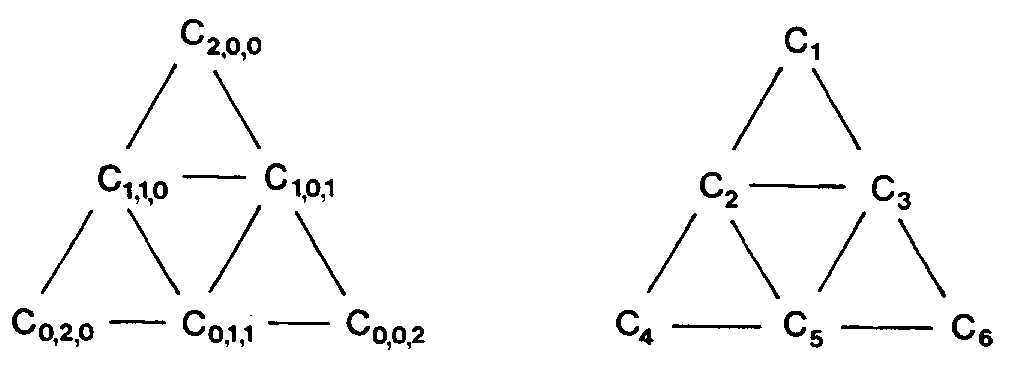
\includegraphics[width=.9\linewidth]{graf.png}
\end{center}

Če razpišemo sedaj polinom glede na spremenljivko $r$ dobimo:

\begin{align}
p(r,s,t) &= \sum_{i=0}^{2}\sum_{j=0}^{i}c_{2-i,i-j,j}r^{2-i}s^{i-j}t^j \nonumber \\ \nonumber
&= r^2\sum_{j=0}^{0}c_{2,-j,j}s^{-j}t^j + r\sum_{j=0}^{1}c_{1,1-j,j}s^{1-j}t^j + \sum_{j=0}^{2}c_{0,2-j,j}s^{2-j}t^j \\ \nonumber
&= r^2(c_1) + r(c_2s+c_3t) + (c_4s^2+c_5st+c_6t^2)\\ \nonumber
&= r^2(c_1+\frac{s}{r}c_2+\frac{t}{r}c_3+\frac{s^2}{r^2}c_4+\frac{st}{r^2}c_5+\frac{t^2}{r^2}c_6) \\ \nonumber
&= r^2(\frac{s}{r}(c_2+\frac{s}{r}c_4+\frac{t}{r}c_5)+\frac{t}{r}(\frac{t}{r}c_6+c_3)+c_1) \nonumber
\end{align}

Tako zapisan polinom lahko sedaj evaluiramo z manj množenji, kot če bi izvedli de Casteljoujev algoritem.
Tu je potrebno biti pozoren na to, da ne delimo z $0$. Temu se lahko izognemo tako, da ločimo primere glede na to, kje v kontrolnem trikotniku se nahajamo. Ločimo $3$ primere kot je prikazano na sliki.

\begin{center}
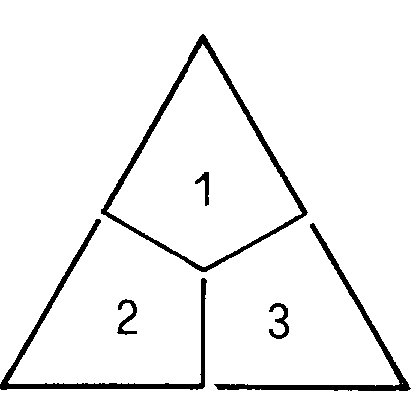
\includegraphics[width=.3\linewidth]{graf1.png}
\end{center}
Posamezne regije so določena na sledeč način
\begin{enumerate}
\item  $r \geq s, r \geq t$
\item $s > r, s \geq t$
\item $t>r, t>s$
\end{enumerate}

S pravilno izbiro regije poskrbimo, da ne delimo z $0$, hkrati pa se izognemo še deljenju z zelo majhnimi števili, ki bi jih dobili pri baricentričnih koordinatah blizu roba.

Zgornji primer lahko posplošimo na polinome poljubnih stopenj.

\begin{algoritm}
\label{MBB}[VS algoritem]
Naj bo p polinom stopnje $d$ podan v MBB obliki, ter naj bodo $ r,s,t$ baricentirčne koordinate točke, za katere velja $r \geq s,r \geq t$, tedaj lahko s sledečim algoritmom izračunamo vrednost polinoma p v točki $(r,s,t)$
\begin{lstlisting}[escapeinside={(*}{*)}]
sr = s/r,	 tr= s/r
A = (*$c_{0,d,0}$*);
for i = 1:d
    B = (*$c_{0,d-i,i}$*)
    for j = i:-1:1
        B = B*tr + (*$c_{i-j+1,d-i,j-1}$*);
    end
    A = A *sr +B;
end
p(r,s,t) = A(*$r^d$*)
\end{lstlisting}
\end{algoritm}

\begin{trditev}
Algoritem za izračun vrednosti polinoma v MBB obliki potrebuje $(d^2+5d)/2$ množenj.
\end{trditev}
\begin{proof}
Sledimo postopku iz dokaza trditve \ref{decast}.
\end{proof}
Tu je potrebno povedati, da se lahko $r^d$ izračuna hitreje, kot z $d-1$ množenji, torej je samo število operacij v algoritmu še nekoliko manjše. Podobno lahko izpeljemo tudi algoritme za ostala območja.


\vspace{3mm}

Pojavlja se še vprašanje zahtevnosti pretvorbe polinoma v MBB obliko. Če se lotimo naivno in na novo poračunamo vse koeficiente, potem nas ta postopek stane $O(d^3)$ operacij. To povzroči, da je časovna zahtevnost, ki jo potrebujemo za izračun ene točke večja, kot če bi uporabili navadni De Casteljaujev algoritem. Če pa na enem polinomu poračunamo večje število točk, postane VS algoritem bolj učinkovit.

Druga možnost, ki jo imamo pa je ta, da si v naprej poračunamo vrednosti s katerimi moramo množiti koeficiente polinoma. To je potrebno za vsako dimenzijo storiti le enkrat, nato pa za izračun novih koeficientov potrebujemo le še $(d^2+3d-4)/2$ množenj. Temu postopku rečemo VSC algoritem. VSC algoritem je tako vedno bolj učinkovit kot De Casteljaujev algoritem.

De Casteljaujev algoritem deluje na konveksnih kombinacijah, kar je zelo stabilno če so vsi koeficienti nenegatvini. To se v splošnem ne zgodi, a nam konveksnonst vseeno zagotavlja, da bodo vmesne vrednosti omejene z normo začetnih koeficientov. Podobno omejitev pa lahko naredimo tudi pri VS algoritmu. Ker so vsi ulomki, ter spremenljivke $(r,s,t)$ manjše od $1$, velja da so vse vmesne vrednosti manše kot produkt norme koeficientov in števila koeficientov.

\section{Polinom v Taylorjevi vrsti}

Naj bo T trikotnik in naj bo $p$ polinom stopnje $d$ definiran na $T$. Naj bosta $u = x-x_1$ in $v = y-y_1$ določena na tak način. Tu sta $(x_1,y_1)$ koordinati poljubnega ogljišča trikotnika. Polinom $p$ lahko potem zapišemo v Taylorjevi obliki kot 
$$p(u,v) = \sum_{i = 0}^d{\sum_{j=0}^{d-i}{a_{i,j}u^iv^j }}.$$To obliko bomo krajše klicali $TAY$.  Vrednost polinoma $p$ v točki $(u,v)$ lahko izračunamo s sledečim algoritmom.

\begin{algoritm}
Naj bo p polinom stopnje $d$ podan v Taylorjevi obliki. Tedaj lahko s sledečim algoritmom izračunamo vrednost polinoma p v točki $(u,v)$
\begin{lstlisting}[escapeinside={(*}{*)}]

p = (*$a_{0,d}$*)
for i = 1:d
    A = (*$a_{i,d-i}$*)
    for j = 1:i
        A = A * u + (*$a_{i-j,d-i}$*)
    end
    p = p * v + A
end
\end{lstlisting}
\end{algoritm}

\begin{trditev}
Taylorjev algoritem za izračun vrednosti polinoma potrebuje $(d^2+3d)/2$ množenj.
\end{trditev}

\begin{proof}
Sledimo postopku iz dokaza trditve \ref{decast}.
\end{proof}

\section{Primerjava algoritmov}

V spodnji tabeli lahko vidimo primerjavo števila množenj, ki jih posamezen algoritem izvede odvisno od stopnje polinoma.

\begin{center}
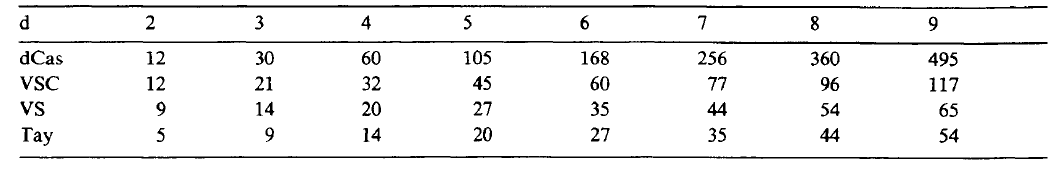
\includegraphics[width=.9\linewidth]{tabelca.PNG}
\end{center}

 Dosedanji algoritmi imajo sledeča števila operacij, pri kateri smo poleg množenj dodali še deljenja, ki pa ne vplivajo bistevno na število operacij, ki jih moramo izvesti.

\begin{align}
(d^3+3d^2+2d)/2& \quad \text{de Casteljau} \nonumber \\
(2d^2+8d)/2& \quad \text{VSC} \nonumber \\
(d^2+5d+4)/2& \quad \text{VS} \nonumber \\
(d^2+3d)/2& \quad \text{Taylor} \nonumber
\end{align}

Tu je jasno vidno, da ima edino de Casteljaujev algoritem kubično zahtevnost, ostali algoritmi pa le kvadratično. Razlika v številu množenj je razvidna v zgornji tabeli. Opazimo tudi, da je Taylorjev algoritem najhitrejši. Vendar nas sama pretvorba iz Bernsteinove ali MBB oblike v Taylorjevo stane preveč, da bi se nam splačalo izvajati Taylorjev algoritem. Zaključimo lahko torej, da je v primeru, ko delamo s polinomi v Bernsteinovi obliki najboljši VSC algoritem.
Na spodnjih grafih lahko vidimo še primerjavo algoritmov glede na časovno zahtevnost v odvisnosti od stopnje polinoma.
\begin{figure}[h]
\centering
\begin{minipage}{.5\textwidth}
\centering
 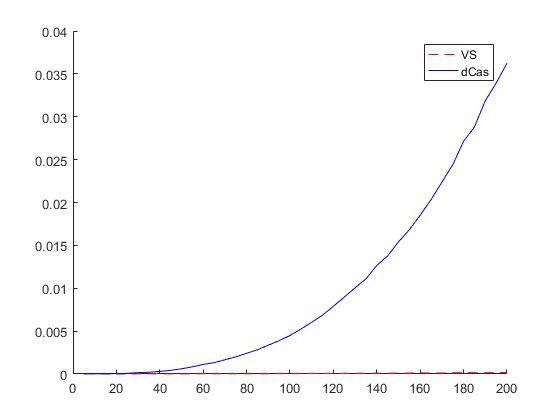
\includegraphics[scale=0.3]{vs}
\label{fig:vs}
\end{minipage}%
\begin{minipage}{.5\textwidth}
\centering
 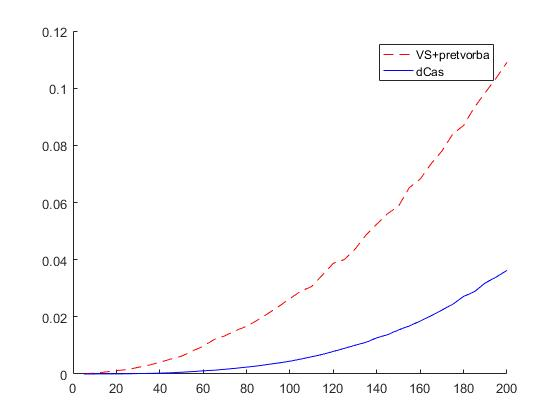
\includegraphics[scale=0.3]{vs_potratn.jpg}
\label{fig:vspot}
\end{minipage}
\end{figure}


 \begin{figure}[h]
\centering
\begin{minipage}{.5\textwidth}
\centering
 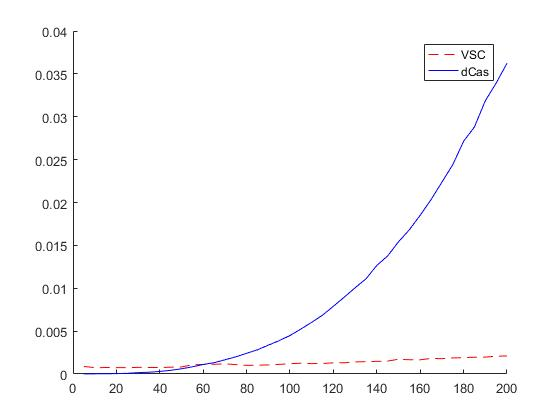
\includegraphics[scale=0.3]{vsc}
\label{fig:vsc}
\end{minipage}
\end{figure}


 \newpage
\section{Gradient}
De Casteljaujev algoritem ne izračuna le vrednosti polynoma $p$ v točki $(r,s,t)$, ampak hkrati vrne tudi gradient v tej točki. Če računamo z MBB algoritmom gradienta ne dobimo. Vendar pa je enostavno dobiti koeficiente $D_rp$ in $D_sp$, ki sta polinoma stopnje $d-1$. Njuni vrednosti izračunamo z VS algoritmov z $d^2 + 3d$ množenj. Torej za vrednost in gradienta potrebujemo skupaj $(3d^2 + 11d + 4)/2$ množenj. Za $d\geq4$ je to hitreje od de Casteljauja. 


\section{Polinomi na tetraedrih}

Naj bo T tetraeder. Za vsako točko $U$ iz $T$ naj bodo $(r,s,t,u)$ pripadajoče baricentrične koordinate glede na $T$.  Naj bo $p$ polinom stopnje $d$ definiran na $T$. Polinom $p$ lahko zapišemo v modificirani Bernstein-Bezierjevi obliki kot 
$$p(r,s,t,u) = \sum_{i = 0}^d{\sum_{j=0}^{i}{\sum_{k = 0}^{j}{c_{d-i,i-j,j-k,k} r^{d-i} s^{i-j} t^{j-k} u^k}}}.$$
Tako podan polinom ima $(d+1)(d+2)(d+3)/6$ koeficientov. Na sliki lahko vidimo te koeficiente v primeru $d=2$.

\begin{center}
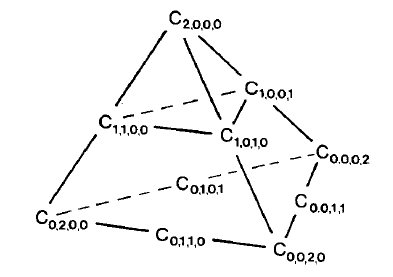
\includegraphics[width=.7\linewidth]{tetraeder.PNG}
\end{center}

Kot v dvodimenzionalnem primeru, uporabimo nekoliko drugačen algoritem, glede na to kje točka $(r, s, t, u)$ leži v tetraedru.
Definiramo štiri regije tetraedra.

\begin{enumerate}
\item $r\geq s, r\geq t, r\geq u$
\item $s\geq r, s\geq t, s\geq u$
\item $t\geq r, t\geq s, t\geq u$
\item $u\geq r,u\geq s, u\geq t$
\end{enumerate}

%zavrtimo točke tako da je računanje efficient

Vrednost polinoma $p$ v točki $(r,s,t,u)$, ki se nahaja v četrti regiji, lahko izračunamo s sledečim algoritmom.

\begin{algoritm}
Naj bo p polinom stopnje $d$ podan v MBB obliki, ter naj bodo $ r,s,t,u$ baricentirčne koordinate točke, za katere velja $u > r,u > s, u>t$, tedaj lahko s sledečim algoritmom izračunamo vrednost polinoma p v točki $(r,s,t,u)$

\begin{lstlisting}[escapeinside={(*}{*)}]
ru = r/u,	 su= s/u	 tu= t/u
A = (*$c_{d,0,0,0}$*);
for i = 1:d
    B = (*$c_{d-i,i,0,0}$*)
    for j = 1:i
        C =  (*$c_{d-i,i-j,j,0}$*)
            for k = 1:j
                C = C * tu + (*$c_{d-i,i-j,j-k,k}$*)
            end
        B = B * ru + C
    end
    A = A * ru + B;
end
p(r,s,t,u) = A(*$u^d$*)
\end{lstlisting}
\end{algoritm}

\begin{trditev}
Zgornji algoritem za izračun vrednosti polinoma potrebuje $(d^3+ 6d^2 + 17d)/6$ množenj.
\end{trditev}

\begin{proof}
Sledimo postopku iz dokaza trditve \ref{decast}.
\end{proof}

Na podoben način lahko izpeljemo tudi algoritme za polinome več spremenljivk.


\begin{thebibliography}{9}

\bibitem{referenca-clanek}
Larry~L.~Schumaker, Wolfgang ~Volk, \emph{Efficient evaluation of multivariate
polynomials}, Computer Aided Geometric Design 3, North-Holland (1986) 149--154.

\end{thebibliography}

\end{document}